In class, we covered one quadratic sort, \emph{selection sort}. Today,
we'll look at the full correctness proof, from beginning to end, for
another sorting algorithm, \emph{insertion sort}. This is somewhat
more complex of a proof, so be sure to follow along carefully!

\section*{Insertion sort%
\TAGS{sorting}}

\begin{minipage}{0.5\textwidth}
\begin{lstlisting}[numbers=left]
void sort(int[] A, int n)
//@requires 0 <= n && n <= \length(A);
//@ensures is_sorted(A, 0, n);
{
  for (int i = 0; i < n; i++)
  //@loop_invariant 0 <= i && i <= n;
  //@loop_invariant is_sorted(A, 0, i);
  {
    int j = i;

    while (j > 0 && A[j-1] > A[j])
    //@loop_invariant 0 <= j && j <= i;
    //@loop_invariant is_sorted(A, 0, j);
    //@loop_invariant is_sorted(A, j, i+1);
    //@loop_invariant le_segs(A,0,j, A,j+1,i+1);
    {
      swap(A, j-1, j);
      j--;
    }
  }
}
\end{lstlisting}
\end{minipage}\hfill%
\begin{minipage}{0.45\textwidth}
\hfill\fbox{%
\parbox{0.96\linewidth}{\smallskip%
  \centering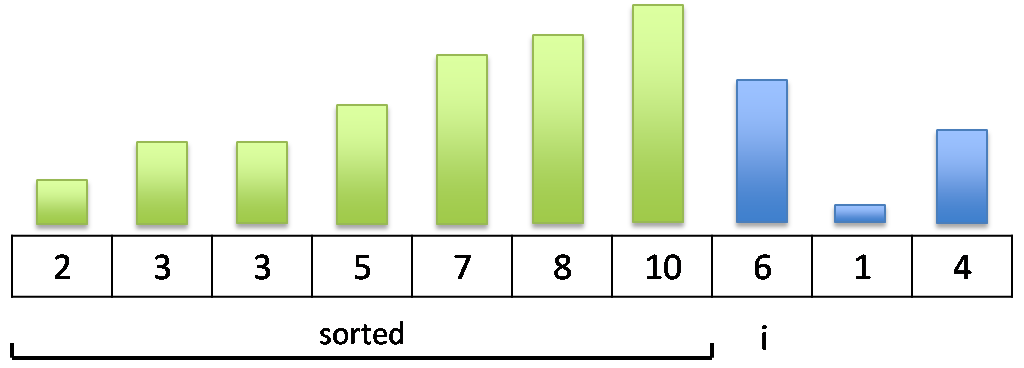
\includegraphics[width=0.98\linewidth]{\img/outer-LI.png}
\par\medskip
\centering\emph{\small Outer loop invariant, schematically}
\par\smallskip
}}%

\vspace{0.8cm}
\hfill\fbox{%
\parbox{0.82\linewidth}{\smallskip%
  \centering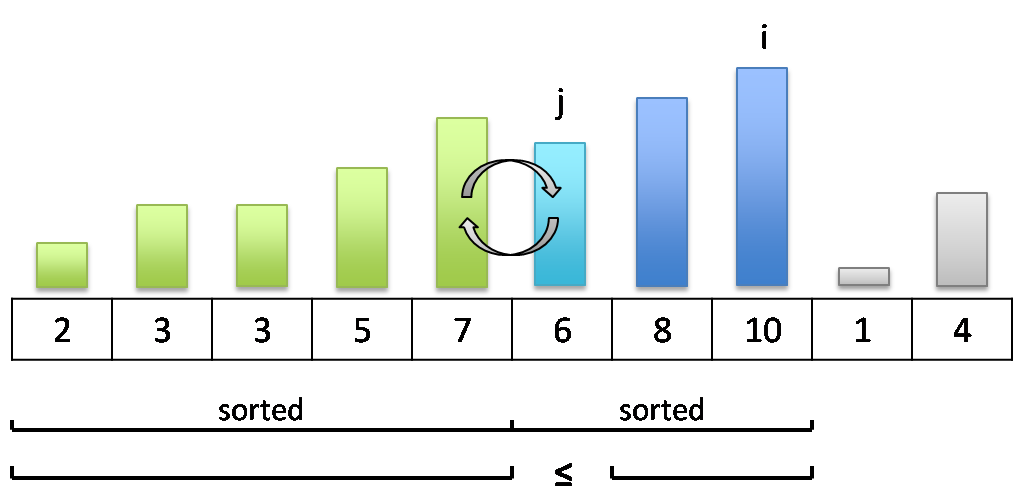
\includegraphics[width=0.98\linewidth]{\img/inner-LI.png}
\par\medskip
\centering\emph{\small Inner loop invariant, schematically}
\par\smallskip
}}
\end{minipage}


To proceed, we need to follow the same four steps we have used all semester to
show correctness for a function with a loop. But when we get to the preservation
step, the loop body is itself a loop, so we must repeat the processes. Below is the structure we will follow.

\begin{enumerate}[1.]
\item Prove outer loop invariants hold INITially
\item Show that outer loop invariants are PREServed
  \begin{enumerate} [(a)]
  \item Prove inner loop invariants hold INITially
  \item Show that inner loop invariants are PREServed
  \item Prove that the inner loop TERMinates
  \item Show that the inner loop invariants and negation of the inner
    loop guard imply the outer loop invariants
  \end{enumerate}
\item Show that the outer loop TERMinates
\item Prove that the postcondition holds on EXIT
\end{enumerate}

\newpage
\begin{enumerate}[1.]
\item\TAGS{correctness, loop-invariant}%
  Prove that, given the preconditions, the outer loop invariants
  INITially hold.

\answerline{Note that $i = 0$ initially, and $n \geq 0$, so the loop
  invariant on line 6 holds.}

\answerline{Moreover, \lstinline'is_sorted(A, 0, 0)' is vacuously true.}

\answerline{}

\answerline{}

\answerline{}

\item\TAGS{correctness, loop-invariant}%
In order to prove that the outer loop invariants are correct, we will need the
negation of the \emph{inner} loop guard along with the preservation and
correctness of the inner loop invariants.
\begin{enumerate}
\itemsep=1ex
\item%
  Assume that the outer loop invariants hold for some iteration of the loop.
  Prove that the \textbf{inner} loop invariants initially hold on this
  iteration. You can imagine you are trying to show the loop invariants are true
  initially for the following block of code:

  \begin{lstlisting}[numbers=left, firstnumber=6]
//@assert 0 <= i && i <= n;
//@assert is_sorted(A, 0, i);

int j=i;

while (j > 0 && A[j-1] > A[j])
//@loop_invariant 0 <= j && j <= i;
//@loop_invariant is_sorted(A, 0, j);
//@loop_invariant is_sorted(A, j, i+1);
//@loop_invariant le_segs(A, 0, j, A, j+1, i+1);
{
  swap(A, j-1, j);
  j--;
}
\end{lstlisting}

\textbf{Line 12:} \answerline{$j= i$ and $i >= 0$, so it holds.}\\[1ex]
\textbf{Line 13:} \answerline{By line 7, and $j=i$, we know \lstinline'is_sorted(A, 0 j)'}\\[1ex]
\textbf{Line 14:} \answerline{(see below)}\\[1ex]
\textbf{Line 15:} \answerline{(see below)}

\begin{solution}\par
\textbf{L14:} When $j=i$, \lstinline'is_sorted(A,j,i+1) == is_sorted(A, i, i+1)', which is a
single element. A single element is, of course, sorted.

\textbf{L15:} Since A[j+1:i+1] == A[i+1:i+1], the second segment passed to
\lstinline'le_segs' is empty. It follows that this vacuously returns
true.
\newpage
\end{solution}

\item%
  Given that the \textbf{inner} loop invariants hold INITially, prove
  that they are PREServed.

\textbf{Line 12:} \answerline{(see below)}\\[1ex]
\textbf{Line 13:} \answerline{}\\[1ex]
\textbf{Line 14:} \answerline{}\\[1ex]
\textbf{Line 15:} \answerline{}

\begin{solution}
This part is complex. Draw an example!

Let $j'$ be the new value of $j$ after one loop.
\begin{description}
\item[L12:] %
 By the loop guard, $j > 0$, so $j' \geq 0$ and $j' = j - 1 < j \leq i$.
\item[L13:] %
  Note that \lstinline'is_sorted(A, 0, j-1)' means elements 0 through
  $j-2$ must be sorted. Since none of these elements are modified in
  the loop, we know this
  is true.
\item[L14:] %
  We know that L15 is initially true, so \lstinline'A[0:j)' <
  \lstinline'A[j+1:i+1)'.  Thus, we know that \lstinline'A[j-1]' <
  \lstinline'A[j+1:i+1]'.  That is, the element to the left of $j$,
  which is larger than $A[j]$ by the loop guard, is smaller than
  everything to the right of $A[j]$ by line 16. Thus, after the swap,
  we know that this is preserved.
\item[L15:] %
  We wish to show \lstinline'A[0:j-1)' < \lstinline'A[j:i+1)'
\end{description}
Note that $A[j-1]$ is now at $j$ by the swap on line 17. $A[j-1]$ is
greater than everything in $A[0:j-1)$ because of the loop invariant on
line 13. Thus, we know that everything in the left segment is smaller
than everything in the right, and the loop invariant holds.
\end{solution}

\item%
  Prove the inner loop TERMinates:
  \answerline{$j$ is a positive quantity that is decreasing to 0.}

We successfully proved the inner loop invariants correct! Now all
that's left is to prove the outer ones.
\newpage
\item%
  Prove the outer loop invariants are PREServed, given that the inner
  loop invariants hold.

  \answerline{(see below)}

  \answerline{}

  \answerline{}
\end{enumerate}

\begin{solution}
  The first loop invariant clearly holds.  For the second one:

  At the end of the inner loop, there are two cases: either $j = 0$ or
  $A[j-1] \leq A[j]$.

  \begin{description}
  \item[Case 1: ]%
    $j = 0$. Then the loop invariant on line 14 proves that
    \lstinline'is_sorted(A,0,i+1)'. Done.
  \item[Case 2: ]%
    $A[j-1] \leq A[j]$.  Then %
    \lstinline'is_sorted(A, 0, j) && A[j-1] < A[j] && is_sorted(A, j, i+1)'
    imply that %
    \lstinline'is_sorted(A, 0, i+1)'.
  \end{description}
\newpage
\end{solution}

\item\TAGS{correctness}%
  Prove that the outer loop TERMinates:
  \answerline{$n-i$ is a constantly decreasing positive quantity.}

\item\TAGS{correctness}%
  Finally, prove that the termination of the outer loop and the
  negation of the outer loop guard prove the postcondition on EXIT.  The
  figure below may be a helpful visualization as you do so.

\answerline{At the end of the loop, $i \leq n$ and $i \geq n$ implies
  $i =n$, so this and}

\answerline{line 7 directly implies the postcondition.}

\answerline{}
\end{enumerate}

\begin{center}
  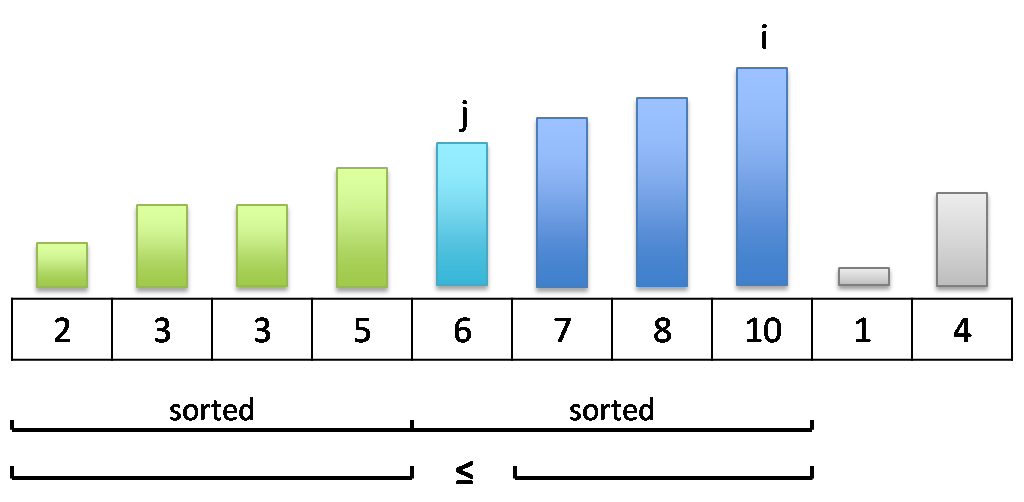
\includegraphics[width=0.6\linewidth]{\img/inner-exit.png}
\end{center}

Whew!  We're done!
